\documentclass[11pt]{amsart}
\usepackage[margin=1.1in]{geometry}
\usepackage[T1]{fontenc}
\usepackage{lmodern}
\usepackage{amssymb,mathtools}
\usepackage{booktabs}
\usepackage{tikz}
\usetikzlibrary{arrows.meta,positioning,shapes.geometric}
\usepackage{xurl}
\usepackage[colorlinks=false,hidelinks]{hyperref}
\numberwithin{equation}{section}
\theoremstyle{plain}
\newtheorem{thm}{Theorem}[section]
\newtheorem{lem}[thm]{Lemma}
\newtheorem{prop}[thm]{Proposition}
\newtheorem{cor}[thm]{Corollary}
\newtheorem{conj}[thm]{Conjecture}
\theoremstyle{definition}
\newtheorem{defn}[thm]{Definition}
\theoremstyle{remark}
\newtheorem{rem}[thm]{Remark}
\newcommand{\N}{\mathbb{N}}
\newcommand{\Z}{\mathbb{Z}}
\newcommand{\R}{\mathbb{R}}
\newcommand{\C}{\mathbb{C}}
\newcommand{\E}{\mathbb{E}}
\renewcommand{\Re}{\operatorname{Re}}
\renewcommand{\Im}{\operatorname{Im}}
\newcommand{\lean}[1]{\texttt{#1}}

\title{The Liouville Function, the Riemann Hypothesis and Chowla's Conjecture}
\author{Deep Bhattacharjee}
\address{Formerly, Electro-Gravitational Space Propulsion Laboratory (EGSPL), Bhubaneswar, Odisha 751030, India; formerly, University of Calcutta (Heramba Chandra College), 23/49 Gariahat Road, Golpark, Kolkata 700029, West Bengal, India}
\email{d.bhattacharjee@erl-forschung.de}
\subjclass[2020]{11N37 (primary); 11M26, 68V20}
\keywords{Liouville function, Chowla conjecture, Riemann hypothesis}


\begin{document}
\begin{abstract}
We prove that the Riemann hypothesis is equivalent to the bound $\sum_{n\le x}\lambda(n)\ll_\varepsilon x^{1/2+\varepsilon}$ for the Liouville function, which gives the one-point case of Chowla's conjecture with a square-root saving, uniformly in arithmetic progressions under the generalised Riemann hypothesis. We prove that correlation estimates on every subset of a set of shifts force each sign pattern to occur with density $2^{-k}$; with the theorems of Tao and Tao--Teräväinen this gives every sign pattern of length at most three its logarithmic density. All elementary steps are checked in Lean~4.
\end{abstract}
\maketitle

\section{Introduction}

The Liouville function $\lambda(n)=(-1)^{\Omega(n)}$, where $\Omega(n)$ counts the prime factors of $n$ with multiplicity, is the simplest arithmetic function whose sign carries the whole difficulty of the distribution of primes. The prime number theorem is equivalent to $\sum_{n\le x}\lambda(n)=o(x)$, and the Riemann hypothesis, as we show in Section~\ref{sec:rh}, is equivalent to $\sum_{n\le x}\lambda(n)\ll_\varepsilon x^{1/2+\varepsilon}$. In 1965 Chowla \cite{Cho65} proposed that $\lambda$ should behave like a random sequence of signs in a much stronger sense.

\begin{conj}[Chowla]\label{conj:chowla}
For every $k\ge1$ and all distinct non-negative integers $h_1,\dots,h_k$,
\begin{equation}\label{eq:chowla}
\frac1N\sum_{n\le N}\lambda(n+h_1)\lambda(n+h_2)\cdots\lambda(n+h_k)\longrightarrow 0\qquad(N\to\infty).
\end{equation}
\end{conj}

The logarithmic form of the conjecture replaces the Cesàro average $\frac1N\sum_{n\le N}$ by $\frac{1}{\log N}\sum_{n\le N}\frac1n$.\footnote{Precisely, we use the normalised weighted mean $\big(\sum_{n\le N}w_n f(n)\big)/\sum_{n\le N}w_n$ with $w_n=1/n$. Since $\sum_{n\le N}1/n=\log N+O(1)$, this is the same as dividing by $\log N$. The logarithmic mean is weaker than the Cesàro mean: by partial summation, a Cesàro mean that tends to zero forces the logarithmic mean to tend to zero, but the converse fails for general bounded sequences. The logarithmic averages are much more convenient for the entropy methods of \cite{Tao16,TT18,TT19}.} The case $k=1$ is the prime number theorem. The case $k\ge2$ is a statement about additive shifts of a multiplicative function, and it is here that the Riemann hypothesis, which is a statement about the multiplicative structure of $\lambda$, loses its grip. The purpose of this paper is to make that boundary exact: to prove in full what the zeros of $\zeta$ and of Dirichlet $L$-functions do give, to combine it with the strongest unconditional theorems, and to check every elementary step by machine.

\subsection{Results}
Write $L(x)=\sum_{n\le x}\lambda(n)$ and $M(x)=\sum_{n\le x}\mu(n)$.

\begin{thm}\label{thm:A}
The following are equivalent.
\begin{enumerate}
\item The Riemann hypothesis.
\item $M(x)\ll_\varepsilon x^{1/2+\varepsilon}$ for every $\varepsilon>0$.
\item $L(x)\ll_\varepsilon x^{1/2+\varepsilon}$ for every $\varepsilon>0$.
\end{enumerate}
Moreover, for every $\theta>1/2$ and every $C$, the bound $|M(N)|\le CN^\theta$ for all $N$ implies $|L(N)|\le C\zeta(2\theta)N^\theta$ for all $N$.
\end{thm}

\begin{cor}[one-point Chowla with square-root saving]\label{cor:onepoint}
Assume the Riemann hypothesis. Then for every $\varepsilon>0$, uniformly in $0\le h\le N$,
\[
\frac1N\sum_{n\le N}\lambda(n+h)\ll_\varepsilon N^{-1/2+\varepsilon}.
\]
\end{cor}

\begin{thm}\label{thm:B}
Assume the generalised Riemann hypothesis for all Dirichlet $L$-functions. For every $\varepsilon>0$, uniformly in $q\ge1$, $(a,q)=1$ and $x\ge1$,
\[
\sum_{\substack{n\le x\\ n\equiv a\ (\mathrm{mod}\ q)}}\lambda(n)\ll_\varepsilon q^{\varepsilon}x^{1/2+\varepsilon}.
\]
\end{thm}

For a finite set $H\subset\N$ of shifts and signs $\epsilon=(\epsilon_h)_{h\in H}\in\{\pm1\}^H$ we say that $n$ has pattern $(H,\epsilon)$ if $\lambda(n+h)=\epsilon_h$ for every $h\in H$.

\begin{thm}[sign patterns from correlations]\label{thm:C}
Let $(w_n)_{n\ge1}$ be positive weights and let $\E^w_N f=\sum_{n\le N}w_nf(n)\big/\sum_{n\le N}w_n$. Let $H$ be a finite set of shifts with $|H|=k$. If
$\E^w_N\prod_{h\in S}\lambda(n+h)\to0$ for every non-empty $S\subseteq H$, then for every $\epsilon\in\{\pm1\}^H$
\[
\E^w_N\,\mathbf 1\big[n\text{ has pattern }(H,\epsilon)\big]\longrightarrow 2^{-k}.
\]
\end{thm}

\begin{cor}\label{cor:three}
Every sign pattern of length $k\le3$ occurs among $(\lambda(n+h))_{h\in H}$ with logarithmic density $2^{-k}$. Under the Riemann hypothesis, each single sign $\lambda(n+h)=\pm1$ occurs with natural density $1/2$, with error $O_\varepsilon(N^{-1/2+\varepsilon})$.
\end{cor}

The first statement of Corollary~\ref{cor:three} combines Theorem~\ref{thm:C} with Tao's logarithmic two-point theorem \cite{Tao16} and the odd-order theorem of Tao and Teräväinen \cite{TT18,TT19}; the consequence itself is implicit in their work, and our contribution is a complete, machine-checked reduction. The implications are summarised in Figure~\ref{fig:map}.

\begin{figure}[t]
\centering
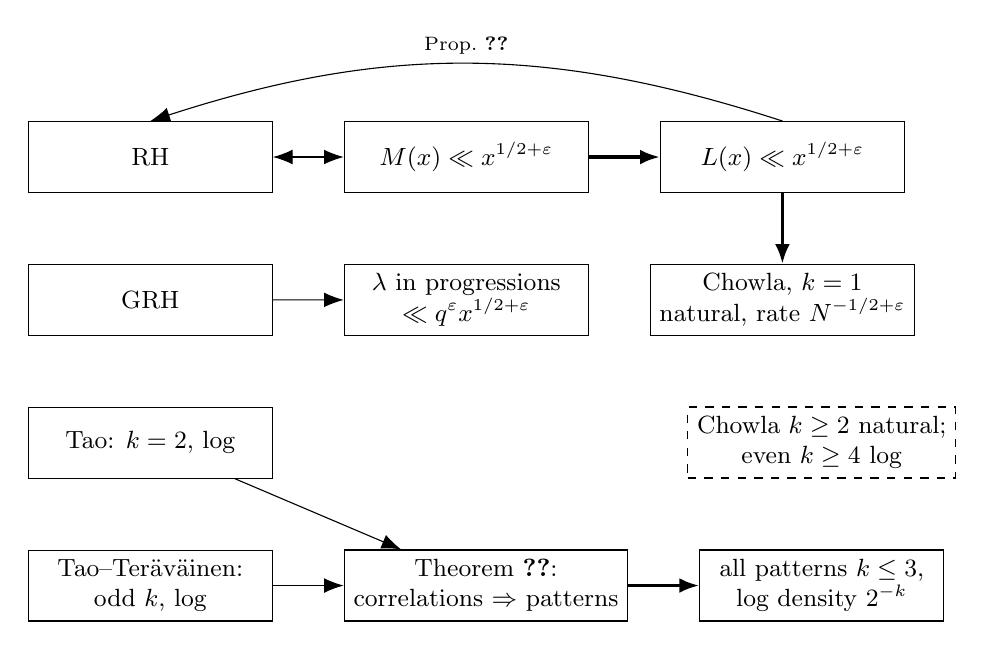
\begin{tikzpicture}[
  box/.style={draw, rectangle, minimum width=31mm, minimum height=9mm, align=center, font=\small},
  dbox/.style={draw, dashed, rectangle, minimum width=31mm, minimum height=9mm, align=center, font=\small},
  lean/.style={-{Latex[length=2.5mm]}, very thick},
  cite/.style={-{Latex[length=2.5mm]}, thin},
  node distance=9mm and 9mm]
\node[box] (rh) {RH};
\node[box, right=of rh] (m) {$M(x)\ll x^{1/2+\varepsilon}$};
\node[box, right=of m] (l) {$L(x)\ll x^{1/2+\varepsilon}$};
\node[box, below=of l] (c1) {Chowla, $k=1$\\ natural, rate $N^{-1/2+\varepsilon}$};
\node[box, below=of rh] (grh) {GRH};
\node[box, below=of m] (ap) {$\lambda$ in progressions\\ $\ll q^\varepsilon x^{1/2+\varepsilon}$};
\node[box, below=of grh] (tao) {Tao: $k=2$, log};
\node[box, below=of tao] (tt) {Tao--Teräväinen:\\ odd $k$, log};
\node[box, right=of tt] (pat) {Theorem~\ref{thm:C}:\\ correlations $\Rightarrow$ patterns};
\node[box, right=of pat] (p3) {all patterns $k\le3$,\\ log density $2^{-k}$};
\node[dbox, above=of p3] (gap) {Chowla $k\ge2$ natural;\\ even $k\ge4$ log};
\draw[{Latex[length=2.5mm]}-{Latex[length=2.5mm]}, thin] (rh) -- (m);
\draw[lean] (m) -- (l);
\draw[cite] (l.north) to[bend right=18] node[above, font=\scriptsize]{Prop.~\ref{prop:converse}} (rh.north);
\draw[lean] (l) -- (c1);
\draw[cite] (grh) -- (ap);
\draw[cite] (tao) -- (pat);
\draw[cite] (tt) -- (pat);
\draw[lean] (pat) -- (p3);
\end{tikzpicture}
\caption{The implications proved here. Thick arrows are checked in Lean~4 with only the standard axioms; thin arrows are proved in the text or are the cited theorems of \cite{Tao16,TT18,TT19}. No arrow leads into the dashed box: no known implication from RH or GRH reaches the two-point correlation with Cesàro averaging, nor the even-order logarithmic correlations of order at least four.}
\label{fig:map}
\end{figure}

\subsection{What remains}
Conjecture~\ref{conj:chowla} for $k\ge2$ with Cesàro averaging, and its logarithmic form for even $k\ge4$, are not proved here and are not known to follow from the Riemann hypothesis or from the generalised Riemann hypothesis. Section~\ref{sec:parity} explains why the zeros of $L$-functions control $\sum\lambda(n)\chi(n)$ but not $\sum\lambda(n)\lambda(n+1)$, and Section~\ref{sec:uncond} lists what is proved without any hypothesis. Every statement we call a theorem is proved in full in this paper, or is quoted from the literature with its source.

\subsection{Formal verification}
The convolution identities of Section~\ref{sec:kernel}, the transfer bound in Theorem~\ref{thm:A}, Corollary~\ref{cor:onepoint} in its qualitative form, Theorem~\ref{thm:C} and Corollary~\ref{cor:three} are formalised in Lean~4 \cite{dMU21} on top of Mathlib \cite{Mathlib20}. The Riemann hypothesis enters the formal development only through the explicit hypothesis \lean{LittlewoodRH}, which is statement (2) of Theorem~\ref{thm:A}, and the theorems of \cite{Tao16,TT18,TT19} enter only as the named hypotheses \lean{TaoTwoPoint} and \lean{TaoTeravainenOdd}. Section~\ref{sec:lean} gives the dictionary.

\section{The square kernel}\label{sec:kernel}

All arithmetic functions are functions $\N_{\ge1}\to\Z$ with Dirichlet convolution $(f*g)(n)=\sum_{ab=n}f(a)g(b)$ and unit $\delta(n)=[n=1]$. We write $\mathbf 1(n)=1$, so that $\mu*\mathbf 1=\delta$.

\begin{lem}\label{lem:kernel}
Let $\sigma=\lambda*\mathbf 1$, that is $\sigma(n)=\sum_{d\mid n}\lambda(d)$. Then $\sigma(n)=1$ if $n$ is a perfect square and $\sigma(n)=0$ otherwise.
\end{lem}

\begin{proof}
Both $\lambda$ and $\mathbf 1$ are multiplicative, hence so is $\sigma$.\footnote{If $f,g$ are multiplicative and $(m,n)=1$, every divisor of $mn$ factors uniquely as $ab$ with $a\mid m$, $b\mid n$, so $(f*g)(mn)=\sum_{a\mid m,\,b\mid n}f(ab)\,g\big(\tfrac ma\cdot\tfrac nb\big)=\sum_{a\mid m}f(a)g(\tfrac ma)\sum_{b\mid n}f(b)g(\tfrac nb)=(f*g)(m)\,(f*g)(n)$, because $(a,b)=(m/a,n/b)=1$.} For a prime power,
\[
\sigma(p^j)=\sum_{i=0}^{j}\lambda(p^i)=\sum_{i=0}^{j}(-1)^i=\begin{cases}1,& j\text{ even},\\ 0,& j\text{ odd}.\end{cases}
\]
If $n=\prod p^{j_p}$, then $\sigma(n)=\prod_p\sigma(p^{j_p})$ is $1$ when every $j_p$ is even, that is when $n=\big(\prod p^{j_p/2}\big)^2$, and $0$ otherwise. Conversely, if $n$ is a square, all exponents are even.
\end{proof}

\begin{lem}\label{lem:conv}
$\lambda=\sigma*\mu$, that is $\lambda(n)=\sum_{d^2\mid n}\mu(n/d^2)$. Consequently, for every real $x\ge1$,
\begin{equation}\label{eq:LM}
L(x)=\sum_{a\le x}\sigma(a)\,M(x/a)=\sum_{d\le\sqrt x}M\!\left(\frac{x}{d^2}\right).
\end{equation}
\end{lem}

\begin{proof}
Convolving $\sigma=\lambda*\mathbf 1$ with $\mu$ and using $\mathbf 1*\mu=\delta$ gives $\sigma*\mu=\lambda$. Summing $\lambda(n)=\sum_{ab=n}\sigma(a)\mu(b)$ over $n\le x$ and grouping by $a$ gives $\sum_{a\le x}\sigma(a)\sum_{b\le x/a}\mu(b)$, which is the first identity. Lemma~\ref{lem:kernel} restricts $a$ to squares $d^2\le x$.
\end{proof}

\section{The Riemann hypothesis and the summatory Liouville function}\label{sec:rh}

\subsection{The transfer bound}

\begin{prop}\label{prop:transfer}
Let $\theta>1/2$ and $C\ge0$. If $|M(N)|\le CN^\theta$ for every integer $N\ge0$, then $|L(N)|\le C\zeta(2\theta)N^\theta$ for every integer $N\ge0$.
\end{prop}

\begin{proof}
By \eqref{eq:LM} with $x=N$, and since $M(m)$ depends only on $\lfloor m\rfloor$ and $\lfloor N/d^2\rfloor\le N/d^2$,
\[
|L(N)|\le\sum_{d^2\le N}C\Big(\frac{N}{d^2}\Big)^{\theta}=CN^\theta\sum_{d^2\le N}d^{-2\theta}\le CN^\theta\sum_{d=1}^\infty d^{-2\theta}=C\zeta(2\theta)N^\theta,
\]
and the series converges because $2\theta>1$.
\end{proof}

This is the step checked in Lean as \lean{liouvilleBound\_of\_mertensBound}. In the formal proof the square restriction is not used through the closed formula on the right of \eqref{eq:LM}; instead $|\sigma(a)|\le1$, $\sigma(a)\ne0\Rightarrow a$ is a square, and the map $d\mapsto d^2$ is injective, which together give the same inequality.

\subsection{Littlewood's theorem}

\begin{thm}[Littlewood; see {\cite[\S14.25]{Tit86}}]\label{thm:littlewood}
If the Riemann hypothesis holds, then $M(x)\ll_\varepsilon x^{1/2+\varepsilon}$ for every $\varepsilon>0$.
\end{thm}

\begin{proof}
Fix $\delta\in(0,1/4)$. Under RH, for $\sigma\ge\frac12+\delta$ and $|t|\ge1$,
\begin{equation}\label{eq:invzeta}
\frac{1}{\zeta(\sigma+it)}\ll_\delta |t|^{\delta}.
\end{equation}
This is \cite[\S14.2]{Tit86}: RH makes $\log\zeta(s)$ holomorphic in $\sigma>1/2$, and the Borel--Carathéodory theorem together with Hadamard's three-circles theorem give $|\log\zeta(\sigma+it)|\le(\log|t|)^{2-2\sigma+\delta}$ for large $|t|$ in that range, whence $|1/\zeta|=\exp(-\Re\log\zeta)\le\exp((\log|t|)^{1-\delta})\ll|t|^\delta$.\footnote{The exponent $2-2\sigma+\delta$ is below $1$ as soon as $\sigma>\frac12+\frac\delta2$, so $\exp\big((\log|t|)^{2-2\sigma+\delta}\big)=|t|^{o(1)}$. For $\sigma\ge 2$ the bound is trivial since $|1/\zeta(s)|\le\zeta(\sigma)\le\zeta(2)$.} On the compact set $\frac12+\delta\le\sigma\le2$, $|t|\le1$, the function $1/\zeta$ is continuous (its only singularities in $\sigma>1/2$ would be zeros of $\zeta$, and the pole of $\zeta$ at $1$ is a zero of $1/\zeta$), so it is bounded there.

Let $x\ge2$ with $x-\frac12\in\Z$, so that $x$ is never an integer, let $c=1+1/\log x$ and $T\ge2$. The truncated Perron formula \cite[Corollary~5.3]{MV07}, applied to $\sum\mu(n)n^{-s}=1/\zeta(s)$ with $|\mu(n)|\le1$, gives
\[
M(x)=\frac{1}{2\pi i}\int_{c-iT}^{c+iT}\frac{x^s}{s\,\zeta(s)}\,ds+O\Big(\frac{x\log x}{T}+1\Big).
\]
The integrand is holomorphic in $\sigma>\frac12$, since under RH $\zeta$ has no zeros there and $1/s$ has its only pole at $0$. By Cauchy's theorem we move the segment to $\sigma_1=\frac12+\delta$. The two horizontal segments contribute, by \eqref{eq:invzeta},
\[
\ll\int_{\sigma_1}^{c}\frac{x^{\sigma}T^{\delta}}{T}\,d\sigma\ll\frac{x\,T^\delta}{T},
\]
and the new vertical segment contributes
\[
\ll x^{\sigma_1}\int_{-T}^{T}\frac{(1+|t|)^{\delta}}{|\sigma_1+it|}\,dt\ll x^{1/2+\delta}\int_0^T(1+t)^{\delta-1}\,dt\ll_\delta x^{1/2+\delta}T^{\delta}.
\]
Choosing $T=x$ gives $M(x)\ll_\delta x^{1/2+2\delta}+\log x\ll x^{1/2+2\delta}$. For an integer $N$, $M(N)=M(N+\frac12)$. Since $\delta$ is arbitrary, the theorem follows.
\end{proof}

\subsection{The converse}

\begin{prop}\label{prop:converse}
If $L(x)\ll_\varepsilon x^{1/2+\varepsilon}$ for every $\varepsilon>0$, then the Riemann hypothesis holds. The same holds with $M$ in place of $L$.
\end{prop}

\begin{proof}
For $\Re s>1$, complete multiplicativity of $\lambda$ gives the Euler product
\[
\sum_{n\ge1}\frac{\lambda(n)}{n^s}=\prod_p\Big(1+\frac1{p^s}\Big)^{-1}=\prod_p\frac{1-p^{-s}}{1-p^{-2s}}=\frac{\zeta(2s)}{\zeta(s)}.
\]
By partial summation, $\sum_{n\le y}\lambda(n)n^{-s}=L(y)y^{-s}+s\int_1^yL(u)u^{-s-1}\,du$. If $L(u)\ll u^{1/2+\varepsilon}$, the integral converges absolutely and locally uniformly in $\Re s>\frac12+\varepsilon$, and $L(y)y^{-s}\to0$ there. Hence the Dirichlet series defines a holomorphic function $F$ on $\Re s>\frac12$, equal to $\zeta(2s)/\zeta(s)$ for $\Re s>1$. By the identity theorem, $F(s)\zeta(s)=\zeta(2s)$ on $\Re s>\frac12$, $s\ne1$. If $\zeta(\rho)=0$ with $\Re\rho>\frac12$, then $\zeta(2\rho)=F(\rho)\zeta(\rho)=0$. But $\Re(2\rho)>1$, where the Euler product shows $\zeta\ne0$. So $\zeta$ has no zeros in $\Re s>\frac12$, and by the functional equation its non-trivial zeros lie on $\Re s=\frac12$. For $M$ the same argument applies to $1/\zeta(s)=\sum\mu(n)n^{-s}$ directly.
\end{proof}

\begin{proof}[Proof of Theorem~\ref{thm:A}]
(1)$\Rightarrow$(2) is Theorem~\ref{thm:littlewood}; (2)$\Rightarrow$(3) is Proposition~\ref{prop:transfer} with $\theta=\frac12+\varepsilon$; (3)$\Rightarrow$(1) and (2)$\Rightarrow$(1) are Proposition~\ref{prop:converse}. The last sentence of the theorem is Proposition~\ref{prop:transfer}.
\end{proof}

\begin{proof}[Proof of Corollary~\ref{cor:onepoint}]
$\sum_{n\le N}\lambda(n+h)=L(N+h)-L(h)$. For $h\le N$, Theorem~\ref{thm:A} gives $|L(N+h)|+|L(h)|\ll_\varepsilon(2N)^{1/2+\varepsilon}+N^{1/2+\varepsilon}\ll N^{1/2+\varepsilon}$. Divide by $N$.
\end{proof}

The Lean theorem \lean{chowlaAt\_single\_of\_liouvilleBound} proves the qualitative statement for any exponent $0\le\theta<1$: the bound $|L(N)|\le CN^\theta$ gives $|\frac1N\sum_{n\le N}\lambda(n+h)|\le 3CN^{\theta-1}$ for $N\ge\max(h,1)$, which tends to $0$.

\begin{rem}
Unconditionally, the best known bound is of the shape
\[
L(x)\ll x\exp\big(-c(\log x)^{3/5}(\log\log x)^{-1/5}\big),
\]
which comes from the Vinogradov--Korobov zero-free region \cite[Chapter~6]{MV07}. Theorem~\ref{thm:A} shows that any saving of a power $x^{-\eta}$ with $\eta>0$ fixed requires a zero-free half-plane $\Re s>1-\eta$, and the square-root saving is exactly RH.
\end{rem}

\section{The generalised Riemann hypothesis and arithmetic progressions}\label{sec:grh}

For a Dirichlet character $\chi$ modulo $q$ put $M_\chi(x)=\sum_{n\le x}\mu(n)\chi(n)$ and $L_\chi(x)=\sum_{n\le x}\lambda(n)\chi(n)$.

\begin{lem}\label{lem:grhmobius}
Assume GRH for $L(s,\chi)$. Then $M_\chi(x)\ll_\delta q^{\delta}x^{1/2+\delta}$ for every $\delta>0$, uniformly in $\chi$ modulo $q$ and $x\ge1$.
\end{lem}

\begin{proof}
Let $\chi$ be induced by the primitive character $\chi^*$ modulo $q^*\mid q$. For $\Re s>1$,
\[
\frac{1}{L(s,\chi)}=\frac{1}{L(s,\chi^*)}\prod_{p\mid q}\big(1-\chi^*(p)p^{-s}\big)^{-1}.
\]
For $\sigma\ge\frac12+\delta$ the finite product is bounded by $\prod_{p\mid q}(1-p^{-1/2})^{-1}\le 4^{\omega(q)}\ll_\delta q^{\delta}$.\footnote{Indeed $(1-p^{-1/2})^{-1}\le(1-2^{-1/2})^{-1}<4$, and $\omega(q)\le(1+o(1))\log q/\log\log q$, so $4^{\omega(q)}=q^{o(1)}$.} Under GRH, the argument of \cite[\S14.2]{Tit86}, carried out for $L(s,\chi^*)$ with the conductor $q^*$ in place of $1$ (see \cite[Chapter~13]{MV07}), gives $1/L(\sigma+it,\chi^*)\ll_\delta (q^*(|t|+2))^{\delta}$ for $\sigma\ge\frac12+\delta$; for principal $\chi$ the pole of $\zeta$ at $s=1$ is a zero of $1/L$ and causes no difficulty. The proof of Theorem~\ref{thm:littlewood} now applies word for word, with the extra factor $q^\delta$ carried through each estimate.
\end{proof}

\begin{proof}[Proof of Theorem~\ref{thm:B}]
Twisting by a completely multiplicative function commutes with Dirichlet convolution: $(f\chi)*(g\chi)=(f*g)\chi$. Hence $\lambda\chi=(\sigma\chi)*(\mu\chi)$ by Lemma~\ref{lem:conv}, and as in \eqref{eq:LM}
\[
L_\chi(x)=\sum_{d\le\sqrt x}\chi(d)^2\,M_\chi(x/d^2).
\]
Lemma~\ref{lem:grhmobius} and the computation of Proposition~\ref{prop:transfer} give $|L_\chi(x)|\ll_\delta \zeta(1+2\delta)\,q^\delta x^{1/2+\delta}$. For $(a,q)=1$, orthogonality of characters gives
\[
\sum_{\substack{n\le x\\ n\equiv a\ (q)}}\lambda(n)=\frac{1}{\varphi(q)}\sum_{\chi\bmod q}\overline{\chi}(a)L_\chi(x),
\]
whose absolute value is at most $\max_\chi|L_\chi(x)|$. Take $\delta=\varepsilon$.
\end{proof}

\begin{rem}
The bound is non-trivial for $q\le x^{1/2-2\varepsilon}$, since the progression has about $x/q$ terms. Unconditionally the Siegel--Walfisz theorem gives a saving by an arbitrary power of $\log x$ only for $q\le(\log x)^A$ \cite[Chapter~11]{MV07}.
\end{rem}

\section{From correlations to sign patterns}\label{sec:patterns}

\begin{proof}[Proof of Theorem~\ref{thm:C}]
For $n\ge1$ and $h\in H$ we have $\lambda(n+h)\in\{\pm1\}$, and for $x,e\in\{\pm1\}$,
\[
\frac{1+e\,x}{2}=\begin{cases}1,& x=e,\\0,&x\ne e.\end{cases}
\]
Therefore
\begin{equation}\label{eq:indicator}
\mathbf 1\big[n\text{ has pattern }(H,\epsilon)\big]=\prod_{h\in H}\frac{1+\epsilon_h\lambda(n+h)}{2}
=2^{-k}\sum_{S\subseteq H}\Big(\prod_{h\in S}\epsilon_h\Big)\prod_{h\in S}\lambda(n+h),
\end{equation}
where we expanded $\prod_{h\in H}(1+y_h)=\sum_{S\subseteq H}\prod_{h\in S}y_h$. The mean $\E^w_N$ is linear, so
\[
\E^w_N\,\mathbf 1[\,\cdot\,]=2^{-k}\sum_{S\subseteq H}\Big(\prod_{h\in S}\epsilon_h\Big)\,\E^w_N\prod_{h\in S}\lambda(n+h).
\]
For $S=\varnothing$ the product is $1$, and $\E^w_N 1=1$ for $N\ge1$ because $\sum_{n\le N}w_n>0$. Every other term tends to $0$ by hypothesis. There are finitely many terms, so the right side tends to $2^{-k}$.
\end{proof}

Taking $w_n=1$ in Theorem~\ref{thm:C}, Conjecture~\ref{conj:chowla} would imply that every sign pattern of every length occurs with natural density $2^{-k}$; the Lean statement is \lean{tendsto\_pattern\_of\_chowla}. The converse also holds: by \eqref{eq:indicator} read backwards,\footnote{Each correlation $\prod_{h\in S}\lambda(n+h)$ equals $\sum_{\epsilon\in\{\pm1\}^S}\big(\prod_{h\in S}\epsilon_h\big)\mathbf 1[n\text{ has pattern }(S,\epsilon)]$, since exactly one $\epsilon$ matches $n$. If every pattern of $S$ has density $2^{-|S|}$, the right side has mean $2^{-|S|}\sum_\epsilon\prod_h\epsilon_h=2^{-|S|}\prod_{h\in S}(1+(-1))=0$ for $S\ne\varnothing$.} equidistribution of all sign patterns of length $k$ gives the Chowla estimates of every order $\le k$. So Conjecture~\ref{conj:chowla} is exactly the statement that $\lambda$ is a normal sequence of signs.

\begin{proof}[Proof of Corollary~\ref{cor:three}]
Let $|H|\le3$ and $w_n=1/n$. Every non-empty $S\subseteq H$ has $|S|\in\{1,2,3\}$. For $|S|\in\{1,3\}$ the logarithmic Chowla estimate is the theorem of Tao and Teräväinen for odd orders \cite{TT18,TT19}; for $|S|=2$ it is Tao's theorem \cite{Tao16}. Theorem~\ref{thm:C} gives the first claim. For the second, take $H=\{h\}$, $w_n=1$; Corollary~\ref{cor:onepoint} and \eqref{eq:indicator} give $\frac1N\#\{n\le N:\lambda(n+h)=e\}=\frac12+\frac e{2N}\sum_{n\le N}\lambda(n+h)=\frac12+O_\varepsilon(N^{-1/2+\varepsilon})$.
\end{proof}

\section{What is proved without hypotheses}\label{sec:uncond}

We record the unconditional theorems that bear on Conjecture~\ref{conj:chowla}. None of them uses the Riemann hypothesis.

\begin{enumerate}
\item \emph{Short intervals.} Matomäki and Radziwiłł \cite{MR16} proved that $\frac1h\sum_{x<n\le x+h}\lambda(n)\to0$ for almost all $x\le X$ as soon as $h=h(X)\to\infty$. This is a one-point statement at every scale, far beyond what RH gives for individual short intervals.
\item \emph{Averaged Chowla.} Matomäki, Radziwiłł and Tao \cite{MRT15} proved that $\sum_{h_1,\dots,h_k\le H}\big|\sum_{n\le X}\lambda(n+h_1)\cdots\lambda(n+h_k)\big|=o(H^kX)$ for $H=H(X)\to\infty$: Conjecture~\ref{conj:chowla} holds for almost all shift vectors.
\item \emph{Sign patterns.} Matomäki, Radziwiłł and Tao \cite{MRT16} proved that all eight sign patterns of length three occur with positive lower natural density, and that at least $k+5$ of the $2^k$ patterns of length $k$ occur with positive density.
\item \emph{Two-point logarithmic Chowla.} Tao \cite{Tao16} proved $\frac1{\log N}\sum_{n\le N}\frac{\lambda(n)\lambda(n+h)}n\to0$ for every $h\ge1$, using \cite{MR16} together with an entropy decrement argument. Helfgott and Radziwiłł \cite{HR21} gave a quantitative version with a different, graph-theoretic method.
\item \emph{Odd orders.} Tao and Teräväinen \cite{TT18,TT19} proved the logarithmic Chowla conjecture for every odd $k$.
\end{enumerate}

Combined with Theorem~\ref{thm:C}, these give Corollary~\ref{cor:three}. The logarithmic case $k=4$ is the first one not covered, and passing from logarithmic to Cesàro averages for $k=2$ is not known either.\footnote{Tao and Teräväinen \cite{TT19} show that the Cesàro two-point statement holds along a set of scales $N$ of logarithmic density one, which is the strongest known result in that direction; the full Cesàro statement for every $N$ is not known.}

\section{Why the zeros do not reach the correlations}\label{sec:parity}

The proof of Theorem~\ref{thm:A} uses only that $\sum_n\lambda(n)n^{-s}=\zeta(2s)/\zeta(s)$ is an Euler product: the Riemann hypothesis tells us where this function is holomorphic, and Perron's formula converts holomorphy into cancellation. The same is true for every twist $\lambda\chi$ (Section~\ref{sec:grh}) and for every twist by $n^{it}$. In each case the object is a multiplicative function, and its Dirichlet series factors over primes.

The correlation $\lambda(n)\lambda(n+1)$ is not multiplicative in $n$, and $\sum_n\lambda(n)\lambda(n+1)n^{-s}$ has no Euler product and no known analytic continuation. Its partial sums are not determined by the zeros of any $L$-function. This is the analytic form of Selberg's parity phenomenon: sieve methods and the distribution of $\lambda$ in progressions of level up to $x^{1-\eta}$, even granting GRH in the form of Theorem~\ref{thm:B}, cannot distinguish integers with an even number of prime factors from those with an odd number along a shifted sequence \cite{FI10}. The entropy decrement method of \cite{Tao16} and the expander method of \cite{HR21} succeed for logarithmic averages because they use the multiplicativity $\lambda(pn)=-\lambda(n)$ at many primes $p$ simultaneously, which is information about $\lambda$ along dilations, not about the zeros of $\zeta$. Sarnak's lectures \cite{Sar11} explain the same boundary from the dynamical side.

For these reasons we do not claim Conjecture~\ref{conj:chowla} for $k\ge2$, under RH or otherwise. What the zeros give is exactly Theorem~\ref{thm:A}, Corollary~\ref{cor:onepoint} and Theorem~\ref{thm:B}.

\section{The Lean formalisation}\label{sec:lean}

The development is in the repository \url{https://github.com/anaxia-research/chawla-rh}, built with Lean~4.35.0 and Mathlib (tag \texttt{v4.35.0}). It contains four files and no \texttt{sorry}, no new axiom and no \texttt{native\_decide}. The command \texttt{\#print axioms} reports, for every theorem in Table~\ref{tab:lean}, only \texttt{propext}, \texttt{Classical.choice} and \texttt{Quot.sound}, the standard axioms of Lean and Mathlib. The Liouville function is Mathlib's \texttt{ArithmeticFunction.liouville}.

\begin{table}[h]
\centering\small
\begin{tabular}{@{}lll@{}}
\toprule
Lean name & Statement & Paper\\
\midrule
\lean{sqKernel\_spec}, \lean{sqKernel\_sq} & $\sigma\in\{0,1\}$, $\sigma\ne0\Rightarrow$ square, $\sigma(d^2)=1$ & Lemma~\ref{lem:kernel}\\
\lean{liouville\_eq\_sqKernel\_mul\_moebius} & $\lambda=\sigma*\mu$ & Lemma~\ref{lem:conv}\\
\lean{summatoryLiouville\_eq} & $L(N)=\sum_{a\le N}\sigma(a)M(N/a)$ & \eqref{eq:LM}\\
\lean{liouvilleBound\_of\_mertensBound} & $M\ll N^\theta\Rightarrow L\ll N^\theta$, $\theta>\frac12$ & Prop.~\ref{prop:transfer}\\
\lean{liouvilleBound\_of\_littlewoodRH} & (2)$\Rightarrow$(3) of Theorem~\ref{thm:A} & Thm.~\ref{thm:A}\\
\lean{chowlaAt\_single\_of\_liouvilleBound} & $L\ll N^\theta$, $\theta<1\Rightarrow$ one-point mean $0$ & Cor.~\ref{cor:onepoint}\\
\lean{chowlaOrder\_one\_of\_littlewoodRH} & Chowla, $k=1$, from \lean{LittlewoodRH} & Cor.~\ref{cor:onepoint}\\
\lean{tendsto\_pattern} & correlations $\Rightarrow$ patterns, any weights & Thm.~\ref{thm:C}\\
\lean{tendsto\_pattern\_of\_chowla} & full Chowla $\Rightarrow$ all patterns & \S\ref{sec:patterns}\\
\lean{logPattern\_le\_three} & patterns $k\le3$, log density & Cor.~\ref{cor:three}\\
\lean{natPattern\_one\_of\_littlewoodRH} & single signs, natural density $\frac12$ & Cor.~\ref{cor:three}\\
\bottomrule
\end{tabular}
\caption{Formalised statements.}
\label{tab:lean}
\end{table}

Three hypotheses appear as explicit propositions and are never assumed silently. \lean{LittlewoodRH} is $\forall\varepsilon>0$, $\exists C$, $\forall N$, $|M(N)|\le CN^{1/2+\varepsilon}$; Theorem~\ref{thm:A} shows it is equivalent to RH, but that equivalence uses Perron's formula and complex analysis of $\zeta$ that Mathlib does not yet contain, so it is proved here on paper only. \lean{TaoTwoPoint} and \lean{TaoTeravainenOdd} state the theorems of \cite{Tao16} and \cite{TT18,TT19} in the notation of the formalisation. The arithmetic progression statement of Theorem~\ref{thm:B} is proved on paper only.

\subsection*{Data availability}
The Lean sources, the build configuration, the output of \texttt{\#print axioms} and the source of this article are in the GitHub repository \url{https://github.com/anaxia-research/chawla-rh}.

\subsection*{Funding}
This research received no external funding.

\subsection*{Conflicts of interest}
The author declares no conflicts of interest.

\begin{thebibliography}{99}

\bibitem{Cho65} S. Chowla, \emph{The Riemann Hypothesis and Hilbert's Tenth Problem}, Mathematics and Its Applications, vol.~4, Gordon and Breach, New York, 1965.

\bibitem{dMU21} L. de Moura and S. Ullrich, \emph{The Lean~4 theorem prover and programming language}, in: Automated Deduction -- CADE 28, Lecture Notes in Comput. Sci. \textbf{12699}, Springer, 2021, 625--635. \href{https://doi.org/10.1007/978-3-030-79876-5_37}{doi:10.1007/978-3-030-79876-5\_37}

\bibitem{FI10} J. Friedlander and H. Iwaniec, \emph{Opera de Cribro}, American Mathematical Society Colloquium Publications \textbf{57}, American Mathematical Society, Providence, RI, 2010.

\bibitem{HR21} H. A. Helfgott and M. Radziwiłł, \emph{Expansion, divisibility and parity}, preprint (2021), \href{https://arxiv.org/abs/2103.06853}{arXiv:2103.06853}.

\bibitem{Mathlib20} The mathlib Community, \emph{The Lean mathematical library}, in: Proceedings of the 9th ACM SIGPLAN International Conference on Certified Programs and Proofs (CPP 2020), ACM, 2020, 367--381. \href{https://doi.org/10.1145/3372885.3373824}{doi:10.1145/3372885.3373824}

\bibitem{MR16} K. Matomäki and M. Radziwiłł, \emph{Multiplicative functions in short intervals}, Ann. of Math. (2) \textbf{183} (2016), 1015--1056. \href{https://doi.org/10.4007/annals.2016.183.3.6}{doi:10.4007/annals.2016.183.3.6}

\bibitem{MRT15} K. Matomäki, M. Radziwiłł and T. Tao, \emph{An averaged form of Chowla's conjecture}, Algebra Number Theory \textbf{9} (2015), 2167--2196. \href{https://doi.org/10.2140/ant.2015.9.2167}{doi:10.2140/ant.2015.9.2167}

\bibitem{MRT16} K. Matomäki, M. Radziwiłł and T. Tao, \emph{Sign patterns of the Liouville and Möbius functions}, Forum Math. Sigma \textbf{4} (2016), e14. \href{https://doi.org/10.1017/fms.2016.6}{doi:10.1017/fms.2016.6}

\bibitem{MV07} H. L. Montgomery and R. C. Vaughan, \emph{Multiplicative Number Theory I: Classical Theory}, Cambridge Studies in Advanced Mathematics \textbf{97}, Cambridge University Press, 2007.

\bibitem{Sar11} P. Sarnak, \emph{Three lectures on the Möbius function, randomness and dynamics}, lecture notes, Institute for Advanced Study, 2011. \url{https://publications.ias.edu/sarnak/paper/512}

\bibitem{Tao16} T. Tao, \emph{The logarithmically averaged Chowla and Elliott conjectures for two-point correlations}, Forum Math. Pi \textbf{4} (2016), e8. \href{https://doi.org/10.1017/fmp.2016.6}{doi:10.1017/fmp.2016.6}

\bibitem{TT18} T. Tao and J. Teräväinen, \emph{Odd order cases of the logarithmically averaged Chowla conjecture}, J. Théor. Nombres Bordeaux \textbf{30} (2018), 997--1015. \href{https://doi.org/10.5802/jtnb.1062}{doi:10.5802/jtnb.1062}

\bibitem{TT19} T. Tao and J. Teräväinen, \emph{The structure of logarithmically averaged correlations of multiplicative functions, with applications to the Chowla and Elliott conjectures}, Duke Math. J. \textbf{168} (2019), 1977--2027. \href{https://doi.org/10.1215/00127094-2019-0002}{doi:10.1215/00127094-2019-0002}

\bibitem{Tit86} E. C. Titchmarsh, \emph{The Theory of the Riemann Zeta-Function}, 2nd ed., revised by D. R. Heath-Brown, Oxford University Press, 1986.

\end{thebibliography}
\end{document}
